\chapter{Resultados e Discussão}
\label{chap_resultados}

\section{Resultados da comparação classificador clássico e quântico}

Os resultados obtidos com o classificador clássico e quântico são apresentados a seguir. As métricas de avaliação utilizadas incluem precisão, \textit{recall}, \textit{F1-score}, acurácia, especificidade e AUC-ROC.

\subsection{Classificador Clássico}

\begin{table}[H]
\centering
\caption{Resultados de treinamento do classificador clássico.}
\begin{tabular}{|c|c|c|c|}
\hline
\textbf{Métrica} & \textbf{Setosa} & \textbf{Versicolor} & \textbf{Virginica} \\ \hline
Precisão (Treino) & 100,00\% & 100,00\% & 73,47\% \\ \hline
Recall (Treino) & 100,00\% & 69,05\% & 100,00\% \\ \hline
F1-score (Treino) & 100,00\% & 81,69\% & 84,71\% \\ \hline
Acurácia (Treino) & \multicolumn{3}{|c|}{88,39\%} \\ \hline
Especificidade (Treino) & \multicolumn{3}{|c|}{94,29\%} \\ \hline
\end{tabular}
\subcaption* {Fonte: Autor.}
\end{table}

\begin{figure}[H]
\centering
\caption{Matriz de confusão de treino para o classificador clássico.}
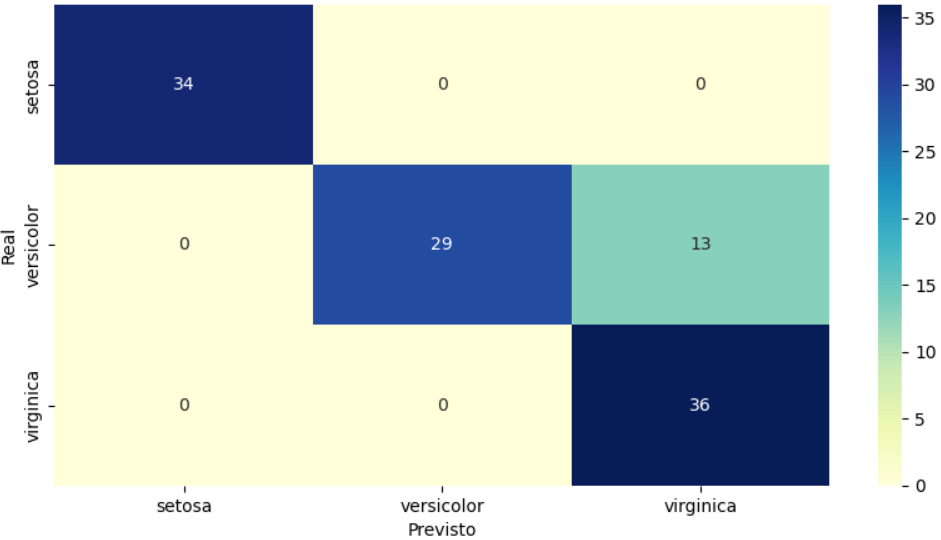
\includegraphics[width=1\textwidth]{imagens/confusion_classic_train.png}
\smallcaption{Fonte: Autor.}
\label{fig:matriz_confusao_classico_treino}
\end{figure}

\begin{table}[H]
\centering
\caption{Resultados de teste do classificador clássico.}
\begin{tabular}{|c|c|c|c|}
\hline
\textbf{Métrica} & \textbf{Setosa} & \textbf{Versicolor} & \textbf{Virginica} \\ \hline
Precisão (Teste) & 100,00\% & 87,50\% & 92,86\% \\ \hline
Recall (Teste) & 100,00\% & 87,50\% & 92,86\% \\ \hline
F1-score (Teste) & 100,00\% & 87,50\% & 92,86\% \\ \hline
Acurácia (Teste) & \multicolumn{3}{|c|}{94,74\%} \\ \hline
Especificidade (Teste) & \multicolumn{3}{|c|}{97,50\%} \\ \hline
\end{tabular}
\subcaption* {Fonte: Autor.}
\end{table}

\begin{figure}[H]
\centering
\caption{Matriz de confusão de teste para o classificador clássico.}
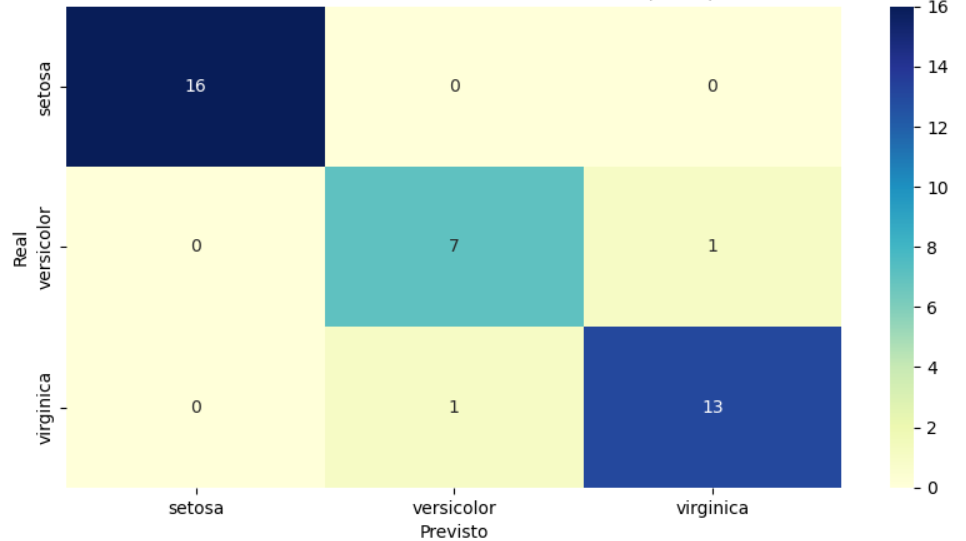
\includegraphics[width=1\textwidth]{imagens/confusion_classic_test.png}
\smallcaption{Fonte: Autor.}
\label{fig:matriz_confusao_classico_teste}
\end{figure}

\subsection{Classificador Quântico}

\begin{table}[H]
\centering
\caption{Resultados de treinamento do classificador quântico.}
\begin{tabular}{|c|c|c|c|}
\hline
\textbf{Métrica} & \textbf{Setosa} & \textbf{Versicolor} & \textbf{Virginica} \\ \hline
Precisão (Treino) & 94,44\% & 70,59\% & 84,00\% \\ \hline
Recall (Treino) & 100,00\% & 85,71\% & 58,33\% \\ \hline
F1-score (Treino) & 97,14\% & 77,42\% & 68,85\% \\ \hline
Acurácia (Treino) & \multicolumn{3}{|c|}{81,25\%} \\ \hline
Especificidade (Treino) & \multicolumn{3}{|c|}{90,24\%} \\ \hline
\end{tabular}
\subcaption* {Fonte: Autor.}
\end{table}

\begin{figure}[H]
\centering
\caption{Matriz de confusão de treino para o classificador quântico.}
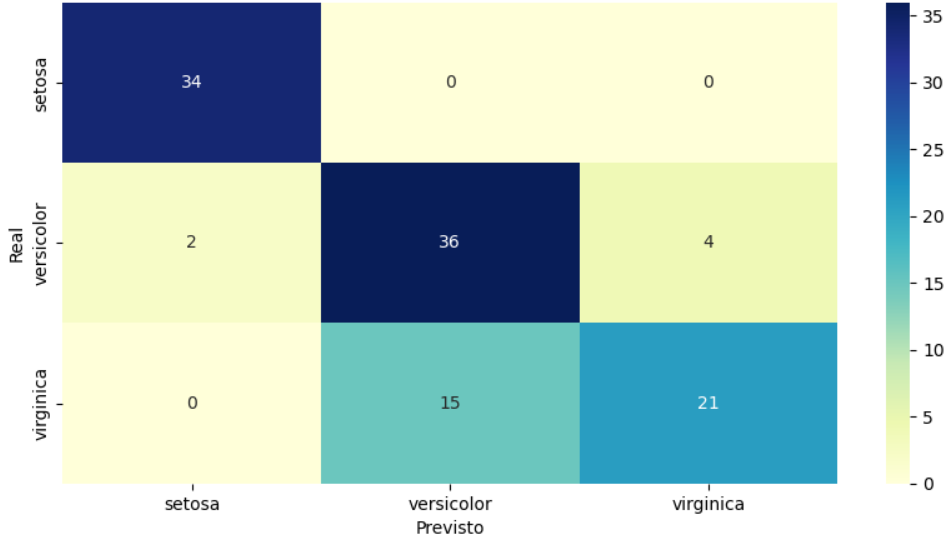
\includegraphics[width=1\textwidth]{imagens/confusion_quantum_train.png}
\smallcaption{Fonte: Autor.}
\label{fig:matriz_confusao_quantico_treino}
\end{figure}

\begin{table}[H]
\centering
\caption{Resultados de teste do classificador quântico.}
\begin{tabular}{|c|c|c|c|}
\hline
\textbf{Métrica} & \textbf{Setosa} & \textbf{Versicolor} & \textbf{Virginica} \\ \hline
Precisão (Teste) & 94,12\% & 53,85\% & 100,00\% \\ \hline
Recall (Teste) & 100,00\% & 87,50\% & 57,14\% \\ \hline
F1-score (Teste) & 96,97\% & 66,67\% & 72,73\% \\ \hline
Acurácia (Teste) & \multicolumn{3}{|c|}{81,58\%} \\ \hline
Especificidade (Teste) & \multicolumn{3}{|c|}{91,82\%} \\ \hline
\end{tabular}
\subcaption* {Fonte: Autor}
\end{table}

\begin{figure}[H]
\centering
\caption{Matriz de confusão de teste para o classificador quântico.}
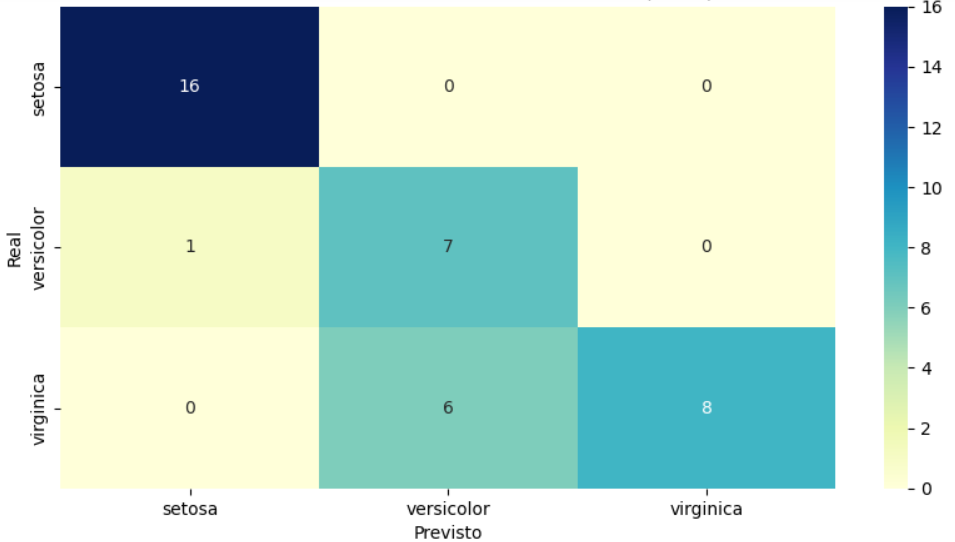
\includegraphics[width=1\textwidth]{imagens/confusion_quantum_test.png}
\smallcaption{Fonte: Autor.}
\label{fig:matriz_confusao_quantico_teste}
\end{figure}

% Número de parâmetros
É importante indicar, porém, que o modelo produzido pelo classificador clássico possuía 584 parâmetros (146 vetores de suporte de quatro componentes cada, somados os três classificadores um-contra-todos, correspondentes a 89 amostras distintas do conjunto de treinamento) enquanto o modelo produzido pelo classificador quântico possuía apenas 12 parâmetros, que são os ângulos das doze portas de rotação do \textit{ansatz}. As duas quantidades, porém, têm naturezas distintas: o número de vetores de suporte retidos depende do tamanho do conjunto de treinamento e do parâmetro de regularização, enquanto os doze ângulos são fixados pela arquitetura do circuito, independentemente da quantidade de dados.

\subsection{Discussão dos Resultados}

Comparando os resultados obtidos, pode-se notar que o classificador clássico e o quântico apresentam desempenhos similares, embora o classificador clássico tenha apresentado uma acurácia geralmente maior. Especificamente, o classificador clássico apresentou uma acurácia de 88,39\% no conjunto de treino e 94,74\% no conjunto de teste, enquanto o classificador quântico obteve uma acurácia de 81,25\% no conjunto de treino e 81,58\% no conjunto de teste.

Uma diferença importante a se destacar é o tempo de treinamento. O classificador clássico levou apenas 0,009 segundos para treinar, enquanto o classificador quântico levou 70,57 segundos. Os dois tempos, porém, não são diretamente comparáveis: o classificador clássico resolve um problema de otimização quadrática sobre os dados, enquanto o tempo do classificador quântico inclui a construção e a execução dos circuitos em cada iteração do COBYLA. Ainda assim, o tempo de treinamento é um aspecto importante a ser considerado ao escolher o classificador a ser usado, especialmente em situações em que esse tempo é um fator crítico.

No que diz respeito à precisão, \textit{recall} e \textit{F1-score}, ambos os classificadores apresentaram desempenho satisfatório na maioria dos casos. No entanto, existem algumas diferenças notáveis. Para a classe \textit{Setosa}, ambos os classificadores obtiveram ótimos resultados, com precisão e \textit{recall} de 100\% na maioria dos casos. No entanto, para as classes \textit{Versicolor} e \textit{Virginica}, o classificador clássico geralmente superou o quântico.

Esses resultados sugerem que, embora o classificador quântico possa ser uma ferramenta valiosa e promissora para problemas de classificação, ainda existem desafios a serem superados, especialmente em termos de eficiência de tempo e desempenho em classes mais difíceis de classificar. Mais pesquisas são necessárias para otimizar ainda mais o desempenho do classificador quântico. Na fase de avaliação de desempenho, a área sob as curvas ROC (AUC-ROC) também foi utilizada como métrica de avaliação dos modelos:

\begin{figure}[H]
\centering
\caption{Curvas ROC de treinamento para o classificador clássico e quântico.}
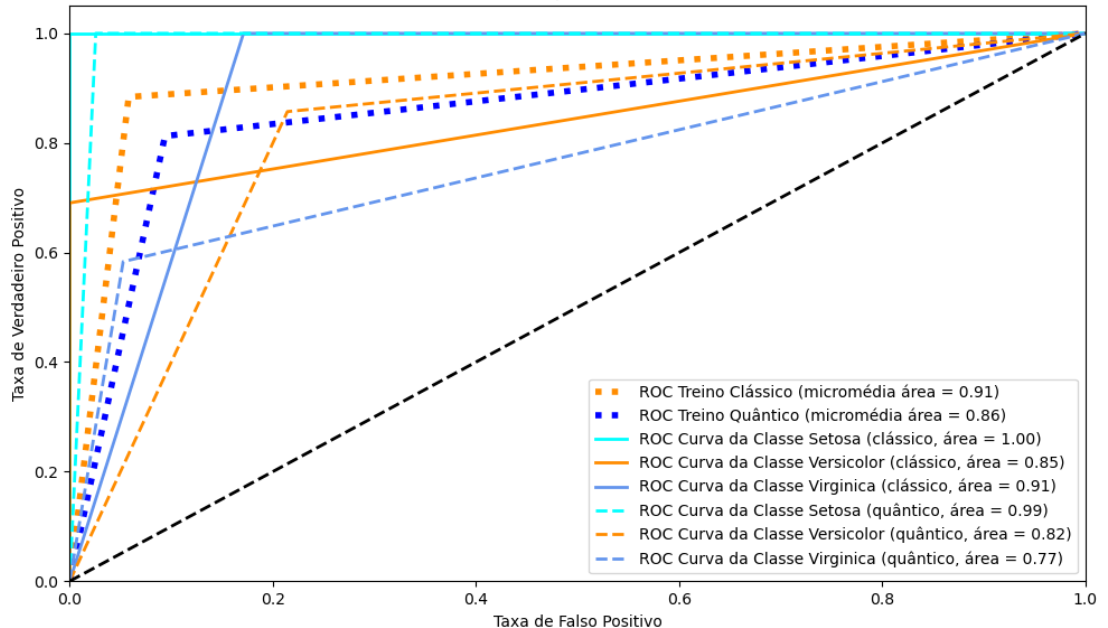
\includegraphics[width=1\textwidth]{imagens/roc_train.png}
\smallcaption{Fonte: Autor.}
\label{fig:roc_train}
\end{figure}

As Curvas de Operação Característica do Receptor (ROC) são utilizadas para avaliar o desempenho de um modelo de classificação, traçando a taxa de verdadeiros positivos em função da taxa de falsos positivos. A Área sob a Curva (AUC - \textit{Area Under the Curve}) é uma medida de quão bem um modelo é capaz de distinguir entre classes.

Na Figura \ref{fig:roc_train}, a curva ROC de treinamento para o classificador clássico apresentou uma micromédia de área igual a 0,91, enquanto o classificador quântico apresentou uma micromédia de área igual a 0,86. Para a classe \textit{Setosa}, ambas as abordagens apresentaram um bom desempenho, com a clássica apresentando área de 1,00 e a quântica de 0,99. No entanto, para as classes \textit{Versicolor} e \textit{Virginica}, o classificador clássico apresentou desempenho superior, com áreas de 0,85 e 0,91, respectivamente, contra 0,82 e 0,77 do quântico.

\begin{figure}[H]
\centering
\caption{Curvas ROC de teste para o classificador clássico e quântico.}
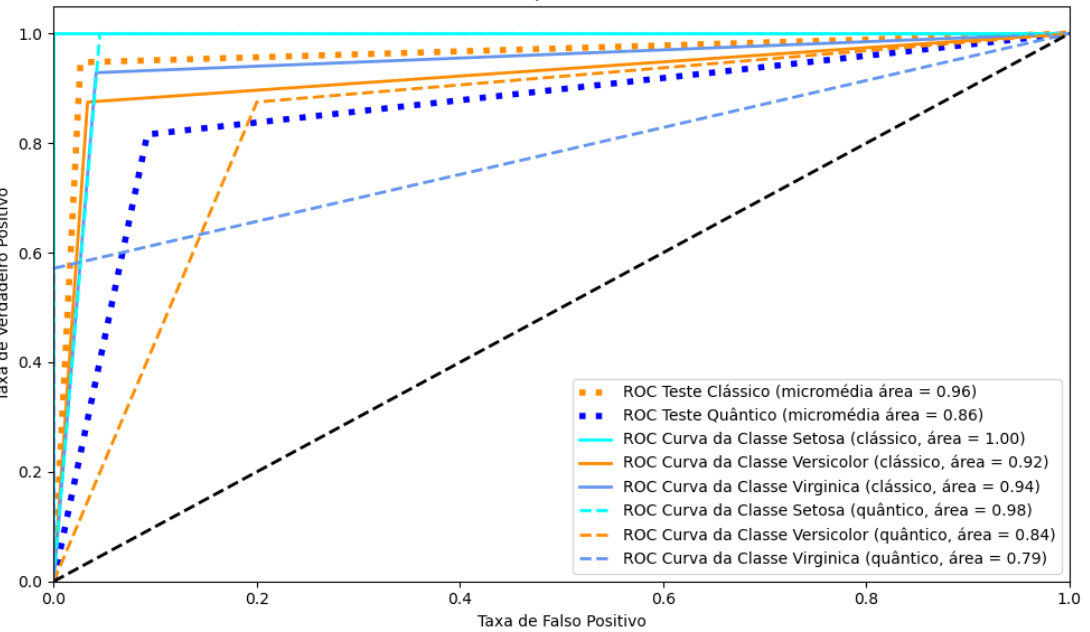
\includegraphics[width=1\textwidth]{imagens/roc_test.png}
\smallcaption{Fonte: Autor.}
\label{fig:roc_test}
\end{figure}

Na Figura \ref{fig:roc_test}, as curvas ROC de teste para o classificador clássico e quântico são apresentadas. O classificador clássico obteve uma micromédia de área igual a 0,96, enquanto o classificador quântico obteve uma micromédia de área igual a 0,86. Ambas as abordagens foram eficazes na classificação da classe \textit{Setosa}, com clássico apresentando uma área de 1,00 e o quântico de 0,98. Na classificação das classes \textit{Versicolor} e \textit{Virginica}, o classificador clássico apresentou melhor desempenho com áreas de 0,92 e 0,94, respectivamente, enquanto o classificador quântico apresentou áreas de 0,84 e 0,79.

É importante notar que essas curvas ROC e os valores de AUC são apenas um dos muitos aspectos a serem considerados na avaliação do desempenho de um classificador. Além deles, a natureza do problema, a importância de falsos positivos versus falsos negativos, a distribuição das classes, entre outros fatores, devem ser levados em consideração.

Esses resultados corroboram com a discussão anterior: o classificador clássico apresenta um desempenho ligeiramente superior ao classificador quântico na maioria dos casos, embora ambos sejam eficazes na distinção entre as classes. A eficácia do classificador quântico é particularmente notável, dada a relativa novidade da computação quântica e suas potencialidades para melhorias futuras.


Em resumo, o presente estudo comparou o desempenho de classificadores clássicos e quânticos na classificação do conjunto de dados Iris. Os resultados indicam que ambos os classificadores são eficazes, com o classificador clássico apresentando um desempenho ligeiramente superior. Entretanto, a eficácia do classificador quântico demonstra o grande potencial da computação quântica na área de aprendizado de máquina.

\section{Avaliação do Comportamento dos Classificadores em Função do Tamanho do Conjunto de Treinamento}

Nesta seção, é avaliado o comportamento dos classificadores clássico e quântico em função do tamanho do conjunto de treinamento. Diversas métricas de desempenho foram avaliadas, incluindo acurácia, especificidade, \textit{recall}, \textit{F1-score} e AUC-ROC. Cada métrica foi avaliada para diferentes tamanhos do conjunto de treinamento, variando de 20\% a 80\% do conjunto de dados total. Os resultados são apresentados a seguir em quatro tabelas, cada uma correspondendo a um classificador e a uma divisão entre treino e teste.

\begin{table}[H]
\centering
\caption{Métricas de treinamento do classificador clássico variando o tamanho do conjunto de treinamento.}
\begin{tabular}{|c|c|c|c|c|c|c|}
\hline
\textbf{Tamanho do Treino} & \textbf{Acurácia} & \textbf{Especificidade} & \textbf{Recall} & \textbf{F1 Score} & \textbf{AUC-ROC} \\ \hline
20\% & 63,3\% & 79,6\% & 63,3\% & 63,3\% & 73,1\% \\ \hline
30\% & 84,4\% & 91,8\% & 84,4\% & 84,4\% & 89,6\% \\ \hline
40\% & 85,0\% & 92,5\% & 85,0\% & 85,0\% & 89,6\% \\ \hline
50\% & 88,0\% & 94,1\% & 88,0\% & 88,0\% & 91,7\% \\ \hline
60\% & 82,2\% & 91,4\% & 82,2\% & 82,2\% & 87,9\% \\ \hline
70\% & 87,6\% & 94,0\% & 87,6\% & 87,6\% & 91,6\% \\ \hline
80\% & 88,3\% & 94,2\% & 88,3\% & 88,3\% & 91,8\% \\ \hline
\end{tabular}
\subcaption* {Fonte: Autor.}
\end{table}

\begin{table}[H]
\centering
\caption{Métricas de teste do classificador clássico variando o tamanho do conjunto de treinamento.}
\begin{tabular}{|c|c|c|c|c|c|c|}
\hline
\textbf{Tamanho do Treino} & \textbf{Acurácia} & \textbf{Especificidade} & \textbf{Recall} & \textbf{F1-score} & \textbf{AUC-ROC} \\ \hline
20\% & 73,3\% & 87,1\% & 73,3\% & 73,3\% & 79,9\% \\ \hline
30\% & 86,7\% & 93,4\% & 86,7\% & 86,7\% & 89,2\% \\ \hline
40\% & 91,1\% & 95,5\% & 91,1\% & 91,1\% & 92,7\% \\ \hline
50\% & 96,0\% & 98,0\% & 96,0\% & 96,0\% & 96,7\% \\ \hline
60\% & 91,7\% & 95,6\% & 91,7\% & 91,7\% & 92,6\% \\ \hline
70\% & 95,6\% & 97,9\% & 95,6\% & 95,6\% & 96,3\% \\ \hline
80\% & 96,7\% & 98,2\% & 96,7\% & 96,7\% & 96,3\% \\ \hline
\end{tabular}
\subcaption* {Fonte: Autor.}
\end{table}

\begin{table}[H]
\centering
\caption{Métricas de treinamento do classificador quântico variando o tamanho do conjunto de treinamento.}
\begin{tabular}{|c|c|c|c|c|c|c|}
\hline
\textbf{Tamanho do Treino} & \textbf{Acurácia} & \textbf{Especificidade} & \textbf{Recall} & \textbf{F1-score} & \textbf{AUC-ROC} \\ \hline
20\% & 76,7\% & 86,3\% & 76,7\% & 76,7\% & 82,5\% \\ \hline
30\% & 80,0\% & 88,5\% & 80,0\% & 80,0\% & 84,9\% \\ \hline
40\% & 81,7\% & 89,8\% & 81,7\% & 81,7\% & 85,3\% \\ \hline
50\% & 74,7\% & 86,0\% & 74,7\% & 74,7\% & 78,8\% \\ \hline
60\% & 70,0\% & 84,0\% & 70,0\% & 70,0\% & 76,2\% \\ \hline
70\% & 73,3\% & 85,8\% & 73,3\% & 73,3\% & 78,9\% \\ \hline
80\% & 80,0\% & 89,6\% & 80,0\% & 80,0\% & 84,7\% \\ \hline
\end{tabular}
\subcaption* {Fonte: Autor.}
\end{table}

\begin{table}[H]
\centering
\caption{Métricas de teste do classificador quântico variando o tamanho do conjunto de treinamento.}
\begin{tabular}{|c|c|c|c|c|c|c|}
\hline
\textbf{Tamanho do Treino} & \textbf{Acurácia} & \textbf{Especificidade} & \textbf{Recall} & \textbf{F1 Score} & \textbf{AUC-ROC} \\ \hline
20\% & 74,2\% & 87,4\% & 74,2\% & 74,2\% & 81,1\% \\ \hline
30\% & 80,0\% & 90,5\% & 80,0\% & 80,0\% & 85,0\% \\ \hline
40\% & 75,6\% & 88,5\% & 75,6\% & 75,6\% & 82,4\% \\ \hline
50\% & 69,3\% & 85,9\% & 69,3\% & 69,3\% & 78,8\% \\ \hline
60\% & 61,7\% & 82,3\% & 61,7\% & 61,7\% & 73,2\% \\ \hline
70\% & 66,7\% & 85,1\% & 66,7\% & 66,7\% & 76,5\% \\ \hline
80\% & 83,3\% & 93,1\% & 83,3\% & 83,3\% & 89,0\% \\ \hline
\end{tabular}
\subcaption* {Fonte: Autor.}
\end{table}

\subsection{Discussão dos Resultados}

Ao analisar os resultados, percebe-se que, de maneira geral, o classificador clássico teve um desempenho superior ao quântico para a maioria das métricas em todos os tamanhos de treinamento. Isto sugere que o modelo clássico pode ser mais adequado para este conjunto de dados. 

Porém, nota-se também que o classificador quântico teve um desempenho consistente em todas as métricas e tamanhos de treinamento, o que indica sua robustez. Com mais otimizações, o classificador quântico pode alcançar e até superar o desempenho do classificador clássico. Portanto, é necessário um estudo mais aprofundado sobre a aplicabilidade e eficácia dos classificadores quânticos.

\section{Resultados dos testes de comparação com computador quântico real}

\begin{table}[H]
\centering
\caption{Resultados de treinamento do classificador clássico.}
\begin{tabular}{|c|c|c|c|}
\hline
\textbf{Métrica} & \textbf{Setosa} & \textbf{Versicolor} & \textbf{Virginica} \\ \hline
Precisão (Treinamento) & 100,00\% & 89,74\% & 94,29\% \\ \hline
Recall (Treinamento) & 100,00\% & 94,59\% & 89,19\% \\ \hline
F1-score (Treinamento) & 100,00\% & 92,11\% & 91,67\% \\ \hline
Acurácia (Treinamento) & \multicolumn{3}{|c|}{94,29\%} \\ \hline
\end{tabular}
\subcaption* {Fonte: Autor}
\end{table}

\begin{table}[H]
\centering
\caption{Resultados de teste do classificador clássico.}
\begin{tabular}{|c|c|c|c|}
\hline
\textbf{Métrica} & \textbf{Setosa} & \textbf{Versicolor} & \textbf{Virginica} \\ \hline
Precisão (Teste) & 100,00\% & 100,00\% & 100,00\% \\ \hline
Recall (Teste) & 100,00\% & 100,00\% & 100,00\% \\ \hline
F1-score (Teste) & 100,00\% & 100,00\% & 100,00\% \\ \hline
Acurácia (Teste) & \multicolumn{3}{|c|}{100,00\%} \\ \hline
\end{tabular}
\subcaption* {Fonte: Autor.}
\end{table}

%\begin{figure}[H]
%\centering
%\caption{Matriz de confusão de teste para o classificador clássico.}
%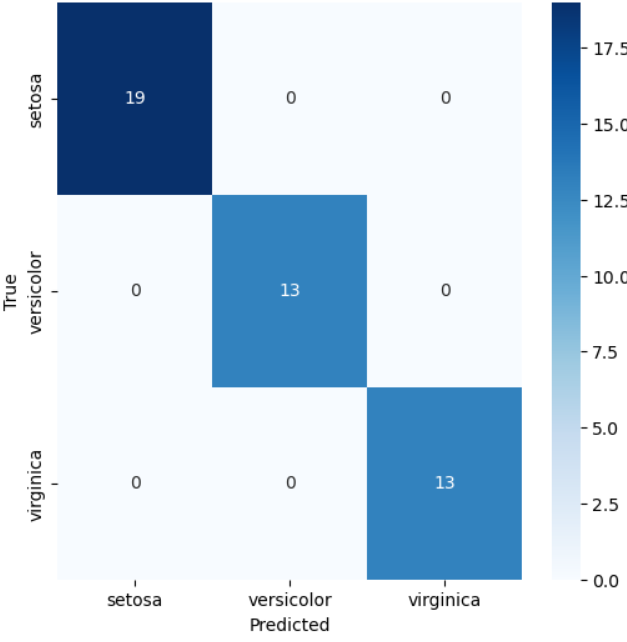
\includegraphics[width=.7\textwidth]{imagens/confusion_classic_test_real.png}
%\subcaption*{Fonte: Autor}
%\label{fig:matriz_confusao_classico_teste_real}
%\end{figure}

\begin{table}[H]
\centering
\caption{Resultados de treinamento do classificador quântico.}
\begin{tabular}{|c|c|c|c|}
\hline
\textbf{Métrica} & \textbf{Setosa} & \textbf{Versicolor} & \textbf{Virginica} \\ \hline
Precisão (Treinamento) & 67,39\% & 45,28\% & 100,00\% \\ \hline
Recall (Treinamento) & 100,00\% & 64,86\% & 16,22\% \\ \hline
F1-score (Treinamento) & 80,52\% & 53,33\% & 27,91\% \\ \hline
Acurácia (Treinamento) & \multicolumn{3}{|c|}{58,10\%} \\ \hline
\end{tabular}
\subcaption* {Fonte: Autor.}
\end{table}

\begin{table}[H]
\centering
\caption{Resultados de teste do classificador quântico.}
\begin{tabular}{|c|c|c|c|}
\hline
\textbf{Métrica} & \textbf{Setosa} & \textbf{Versicolor} & \textbf{Virginica} \\ \hline
Precisão (Teste) & 90,48\% & 52,17\% & 100,00\% \\ \hline
Recall (Teste) & 100,00\% & 92,31\% & 7,69\% \\ \hline
F1-score (Teste) & 95,00\% & 66,67\% & 14,29\% \\ \hline
Acurácia (Teste) & \multicolumn{3}{|c|}{71,11\%} \\ \hline
\end{tabular}
\subcaption* {Fonte: Autor.}
\end{table}

%\begin{figure}[H]
%\centering
%\caption{Matriz de confusão de teste para o classificador quântico real.}
%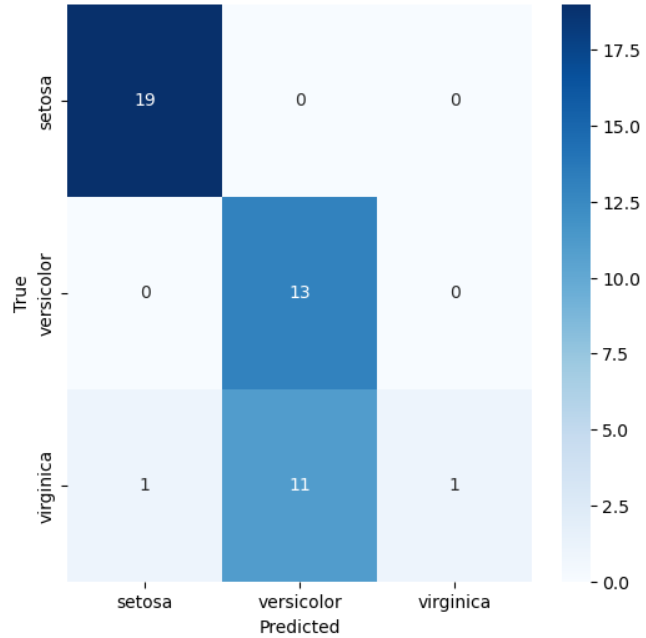
\includegraphics[width=.7\textwidth]{imagens/confusion_quantum_test_real.png}
%\subcaption*{Fonte: Autor}
%\label{fig:matriz_confusao_quantico_teste_real}
%\end{figure}

\subsection{Discussão dos Resultados}

Nesta seção, serão discutidos os resultados obtidos pelo classificador quântico, levando em consideração as limitações e configurações utilizadas.

O classificador quântico foi treinado com configurações específicas, incluindo apenas 1 repetição do \textit{ZFeatureMap}, 1 repetição do \textit{RealAmplitudes} e apenas 20 iterações do COBYLA, o que pode significar que a otimização do modelo foi incompleta. Além disso, utilizou-se 70\% do conjunto de dados como conjunto de treinamento, o que corresponde a 105 amostras de treinamento e 45 de teste. Essas configurações podem afetar o desempenho do classificador quântico, tornando-o limitado em comparação com o classificador clássico.

Ao analisar os resultados obtidos, observa-se que o classificador quântico apresentou desempenho inferior ao classificador clássico em todas as métricas avaliadas. No conjunto de treinamento, a acurácia do modelo quântico foi de 58,10\%, enquanto no conjunto de teste foi de 71,11\%. Essa diferença não indica melhor generalização: as duas amostras têm composições distintas, pois a classe \textit{Setosa}, a única classificada corretamente em todos os casos, representa 42,2\% do conjunto de teste e 29,5\% do de treinamento, enquanto a classe \textit{Virginica}, a de menor \textit{recall}, representa 28,9\% e 35,2\%, respectivamente. Ao ponderar o \textit{recall} por classe obtido no teste pelas proporções do conjunto de treinamento, a acurácia de teste corresponderia a 64,76\%, e a diferença restante não é estatisticamente significativa para esses tamanhos de amostra (teste exato de Fisher, $p = 0{,}15$).

Além disso, as métricas de precisão, \textit{recall} e \textit{F1-score} também foram menores para o classificador quântico em comparação com o classificador clássico. A precisão para a classe \textit{Setosa} foi de 90,48\%, para\textit{Versicolor} foi de 52,17\% e para \textit{Virginica} foi de 100,00\%. O recall para \textit{Setosa} foi de 100,00\%, para \textit{Versicolor} foi de 92,31\% e para \textit{Virginica} foi de 7,69\%. O \textit{F1-score} para \textit{Setosa} foi de 95,00\%, para \textit{Versicolor} foi de 66,67\% e para \textit{Virginica} foi de 14,29\%.

Esses resultados indicam que, com as configurações utilizadas e a quantidade limitada de dados de treinamento, o classificador quântico não foi capaz de capturar efetivamente os padrões nos dados. É importante destacar que o desempenho do classificador quântico pode ser melhorado ao ajustar as configurações, como aumentar o número de repetições do \textit{ZFeatureMap} e do \textit{RealAmplitudes}, aumentar o número de iterações do COBYLA e utilizar uma proporção maior do conjunto de treinamento.

Portanto, nas configurações utilizadas neste estudo, o classificador quântico apresentou desempenho inferior ao do classificador clássico. No entanto, é importante ressaltar que a computação quântica ainda está em estágios iniciais de desenvolvimento e aprimoramento. Com o avanço da tecnologia quântica e a pesquisa contínua nessa área, espera-se que os classificadores quânticos possam superar as limitações atuais e fornecer resultados cada vez mais promissores em tarefas complexas de classificação.